%% Ankur Sinha

%% packages %%
% support for coloured text
\usepackage{color}  

% IPA
\usepackage{tipa}
\usepackage{tikz}
\usepackage{jneurosci}
\usepackage{subfig}  

% Get rid of warnings
\usepackage[default,osfigures,scale=0.95]{opensans}
%\usepackage{lmodern}

% for strike through
\usepackage[normalem]{ulem}

% links, urls, refs
\definecolor{links}{HTML}{2A1B81}
\usepackage{hyperref}
\hypersetup{colorlinks,linkcolor=Green,urlcolor=links}

% graphics
\usepackage{graphicx}

% algorithm
\usepackage{algorithmic}

\usepackage{textcomp}

\usepackage{wrapfig}

%\usepackage[round]{natbib}
% beamer theme
% use defaults for theme
\usetheme{Montpellier}
\usecolortheme[RGB={41,114,65}]{structure}
\logo{
\includegraphics[keepaspectratio,scale=0.25,angle=0]{herts-logo-225x52.jpg}}

\setbeamerfont{caption}{size=\tiny}
\setbeamercolor{alerted text}{fg=Green}

%% title %%
\title[Cortical rewiring]{Loss of sensory input causes rapid structural changes of inhibitory neurons in adult mouse visual cortex}
\subtitle{- UH Biocomputation group journal club -}
\author[Ankur Sinha]{Ankur Sinha}
\institute[UH Biocomputation]{University of Hertfordshire - Biocomputation group}
\date[29/03/2019]{29 March 2019}

%% document begins %%
\begin{document}

%% title frame %%
\begin{frame}
  \titlepage
\end{frame}

\begin{frame}{Outline}
  \small{\tableofcontents}
\end{frame}
\section{Context}
\begin{frame}{I'm looking at:}
  the \alert{functional effects} of cortical rewiring following loss of input.
\end{frame}
\begin{frame}{Plasticity - refresher}
  \begin{figure}
    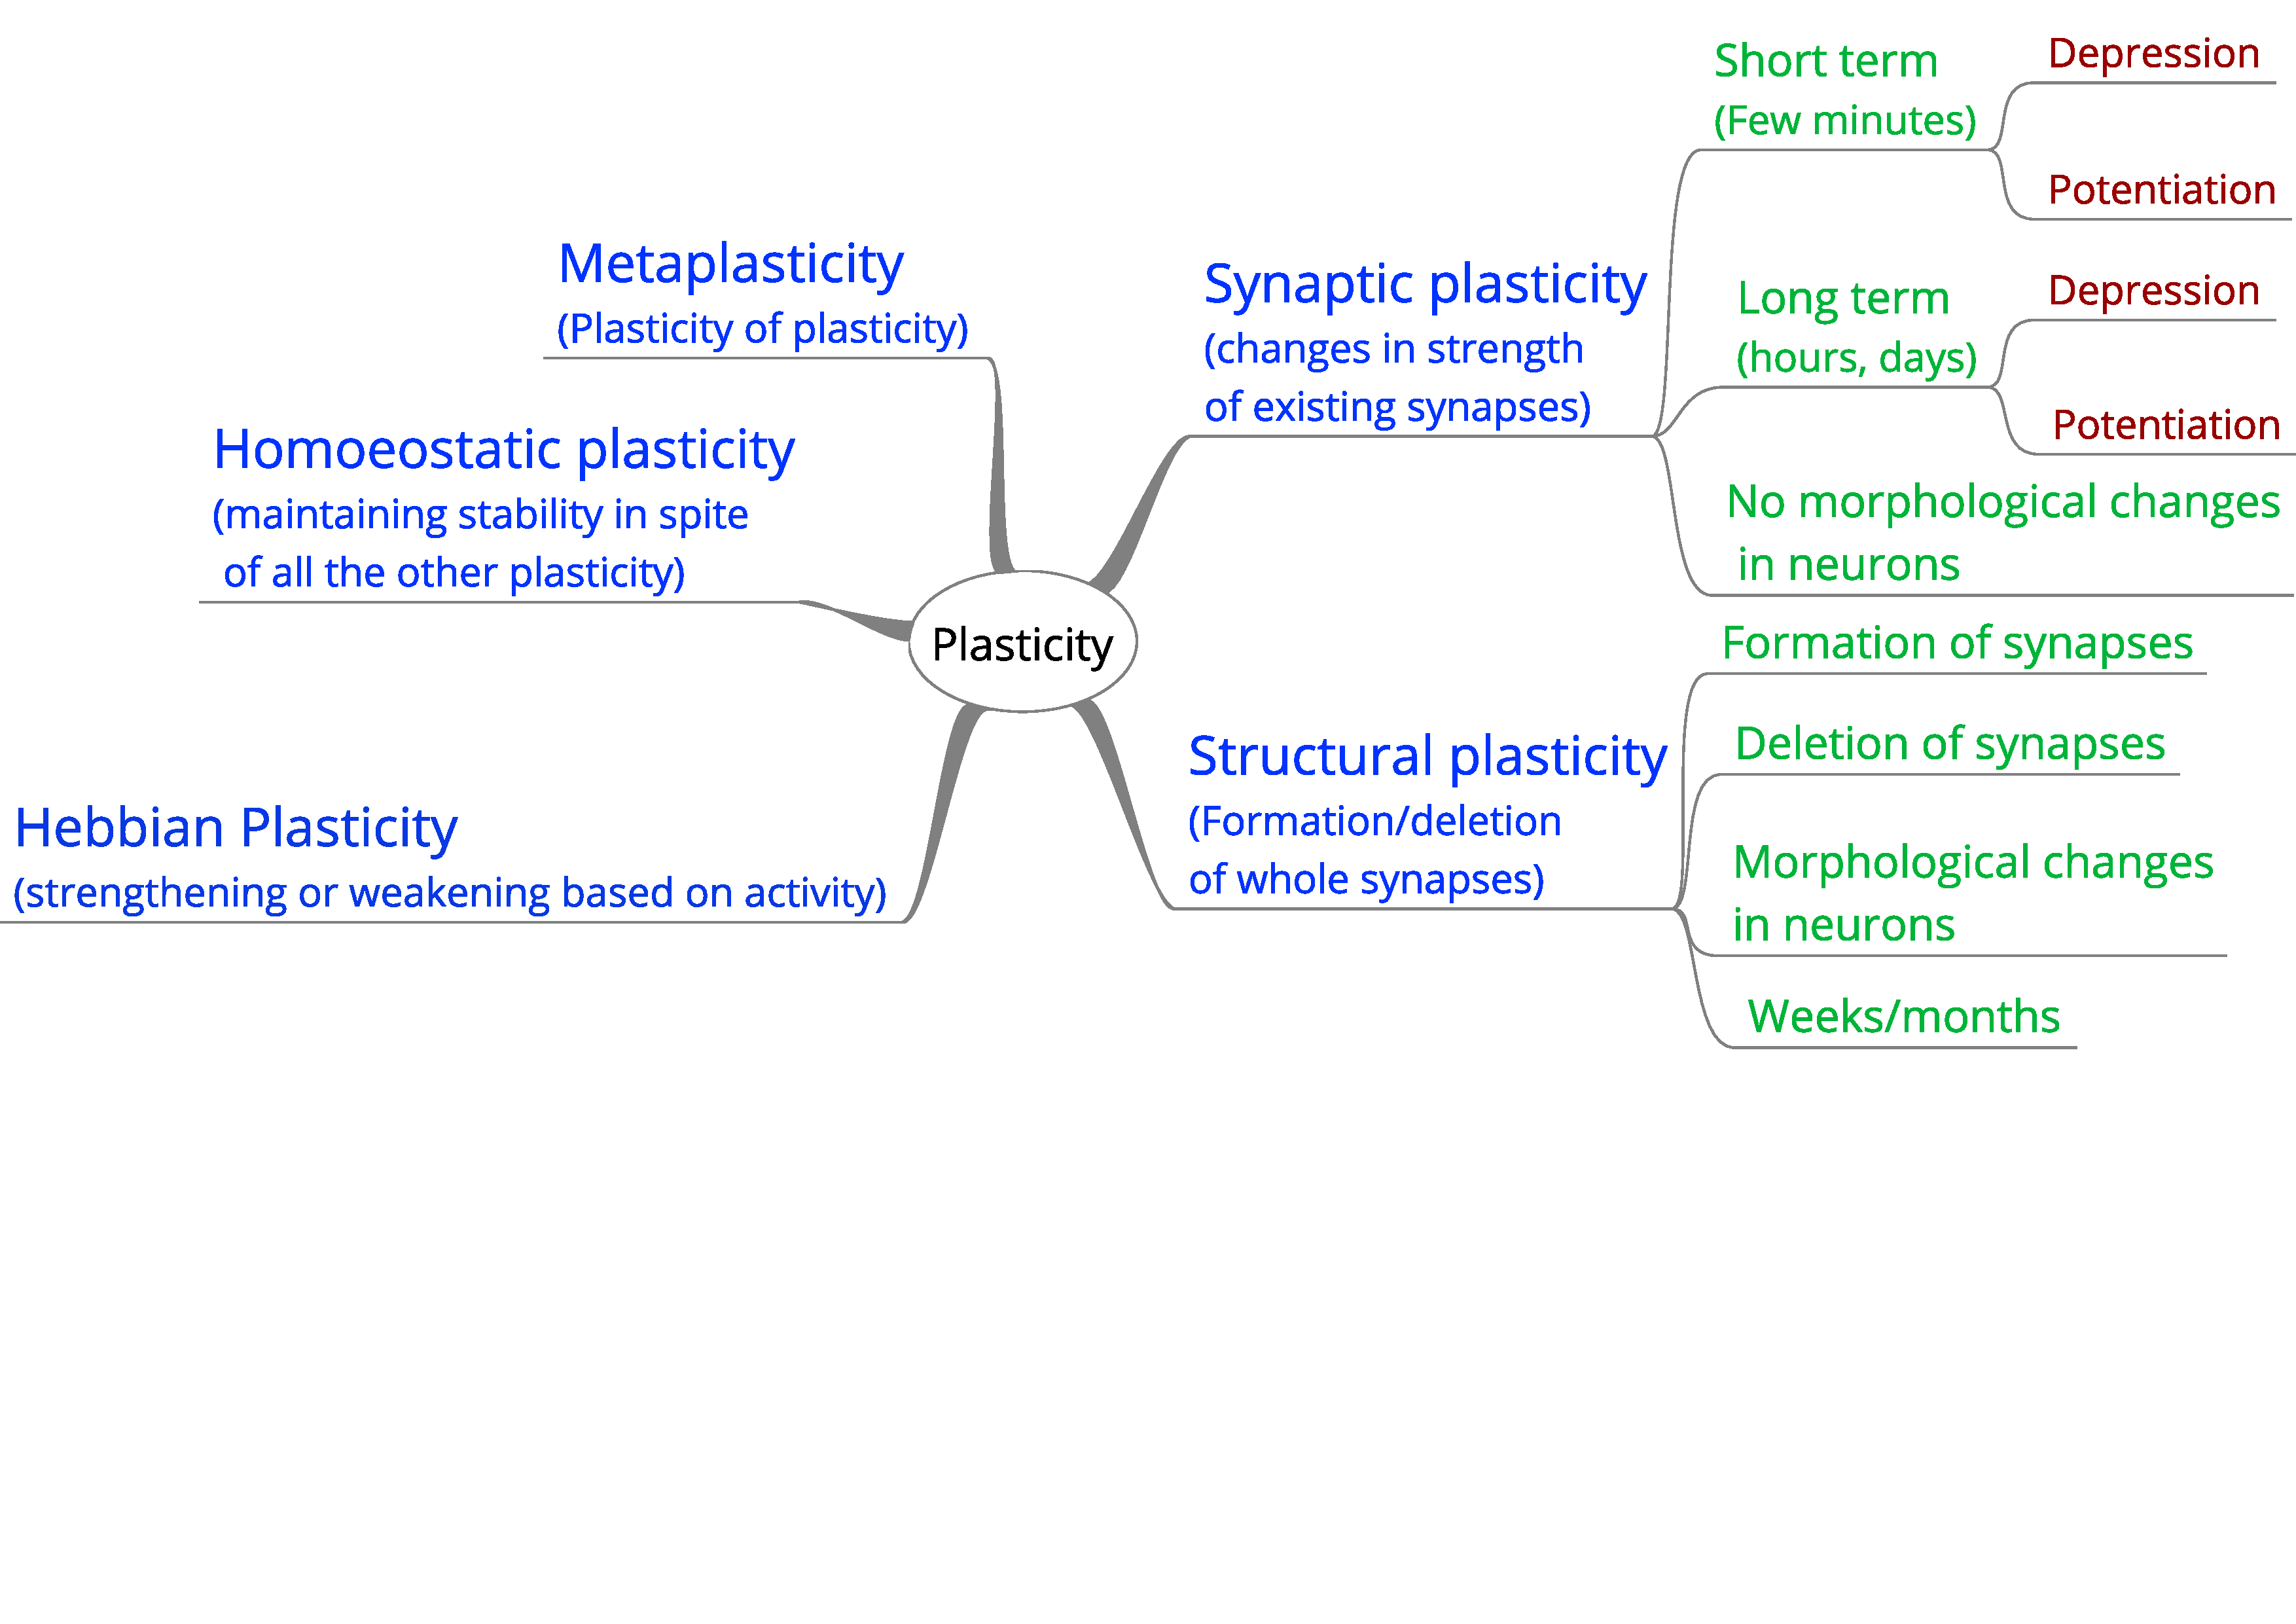
\includegraphics[keepaspectratio,width=\textwidth]{99_images/Plasticity}
  \end{figure}
\end{frame}
\section{Biology}
\begin{frame}{Three papers}
  \begin{itemize}
    \item \href{http://www.nature.com/neuro/journal/v11/n10/abs/nn.2181.html}{Massive restructuring of neuronal circuits during functional reorganisation of adult visual cortex}~\cite{Keck.517}
      \pause
    \item \href{http://www.sciencedirect.com/science/article/pii/S0896627311005642}{Loss of sensory input causes rapid structural changes of inhibitory neurons in adult mouse visual cortex}~\cite{Keck2011869}.
      \pause
    \item \href{http://www.sciencedirect.com/science/article/pii/S0959438815001312}{Adult plasticity and cortical reorganisation after peripheral lesions}~\cite{Sammons2015136}.
    \note[item]{This is a short review paper that summaries the two above}
  \end{itemize}
\end{frame}
\begin{frame}{Model}
  \begin{figure}
    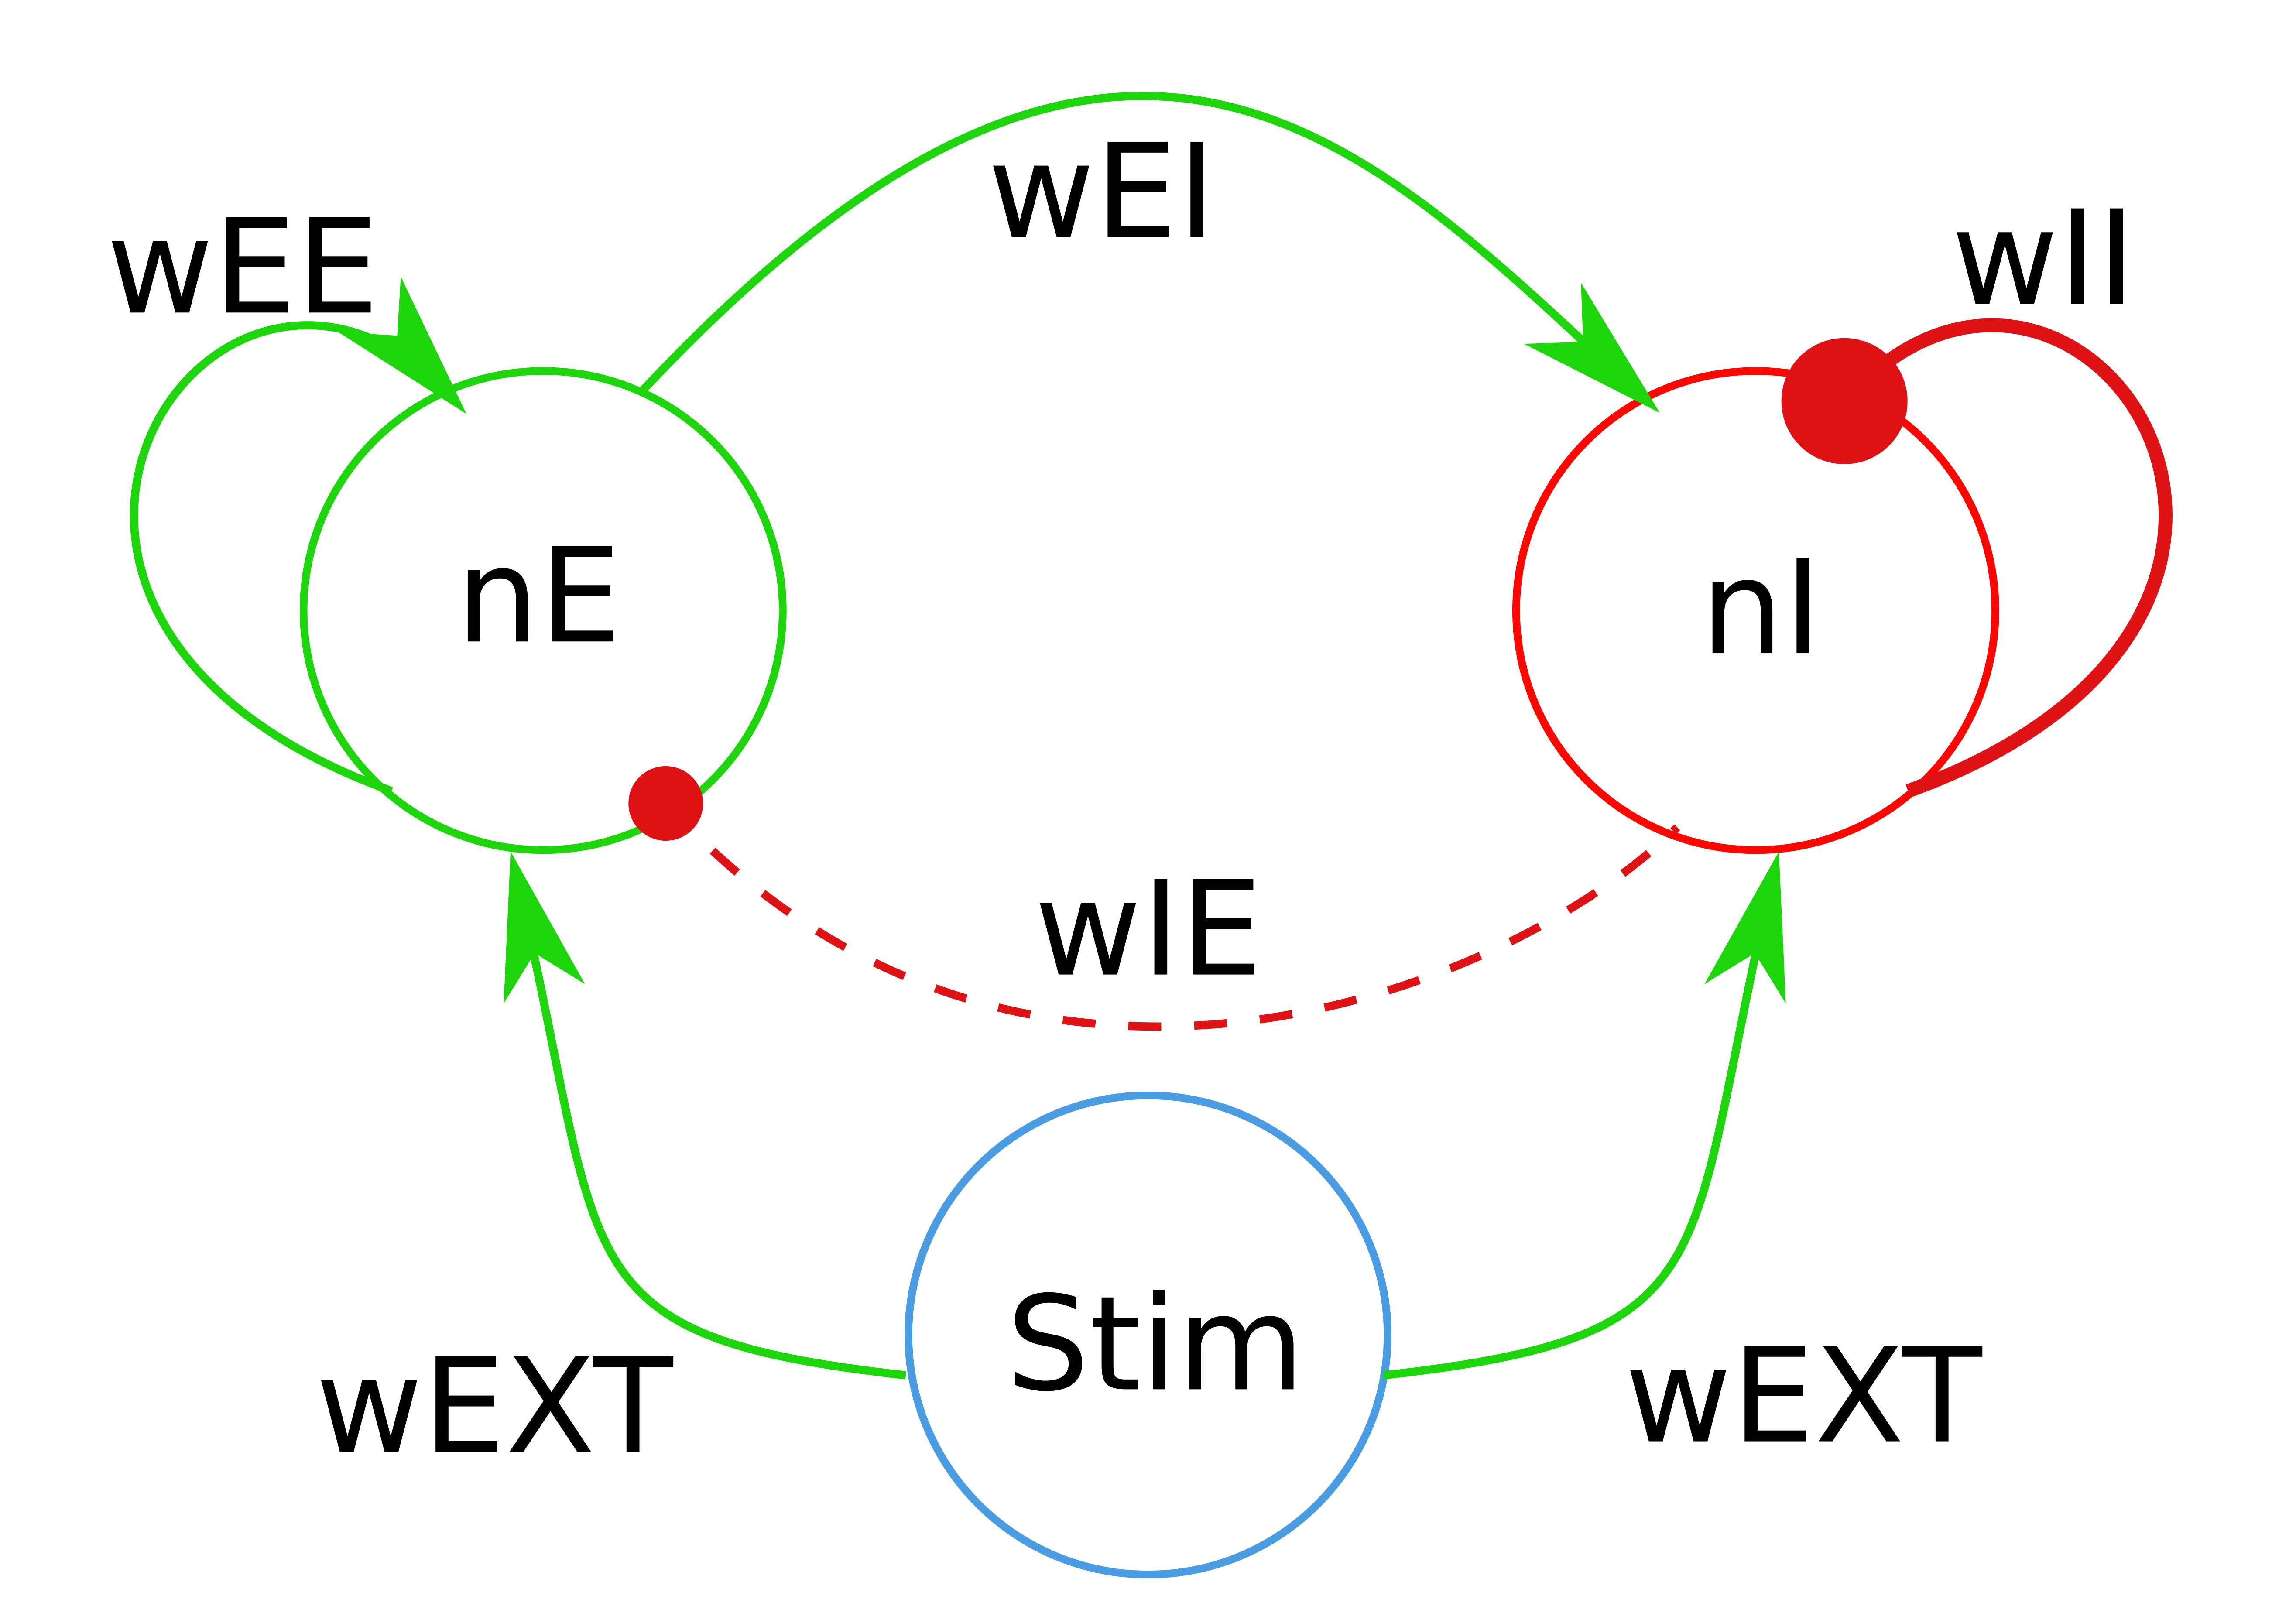
\includegraphics[keepaspectratio,width=0.7\textwidth]{99_images/model-schematic}
    \caption{Model schematic}
  \end{figure}
\end{frame}
\begin{frame}{General observations}
  \begin{itemize}
    \item Peripheral lesion - retinal, for example
    \item Observe the cortex over time
    \note[item]{Depends on what one is looking at, different techniques are used. Could be electrophysiological studies, or imaging}
    \note[item]{Keck et al. use a cranial window technique. There's also a thinning skull technique. Both of which I do not know much about}
    \note[item]{Various species, various cortices, but a lot of work has been done on the visual cortex}
    \begin{itemize}
      \item receive feed-forward input from the lesioned peripheral area
    \end{itemize}
    \pause
  \item \alert{Loss of input} is observed initially after the lesion
    \pause
  \item Gradually, \alert{remapping} occurs, with activity returning to pre-lesion levels
  \note[item]{Several weeks and months}
    \begin{itemize}
      \item \alert{Receptive fields} of deprived neurons \alert{become similar to} receptive fields of cells that are spatially adjacent in the spared cortical regions
      \item \alert{Intra-cortical plasticity}, as little or no reorganisation has been observed in the LGN
      \note[item]{Michael had asked me this at last week's meeting}
    \end{itemize}
  \end{itemize}
\end{frame}
\begin{frame}{Mapping}
  \begin{columns}[c]
    \begin{column}{0.4\textwidth}
      \begin{figure}
        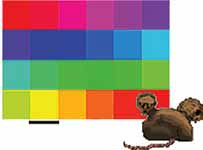
\includegraphics[keepaspectratio,width=\textwidth]{99_images/keck-1-1a}
        \caption{Drifting grating stimuli}
      \end{figure}
    \end{column}
    \pause
    \begin{column}{0.4\textwidth}
      \begin{figure}
        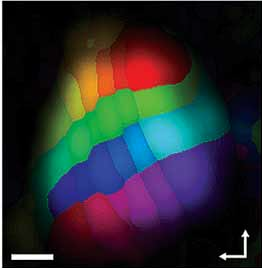
\includegraphics[keepaspectratio,width=\textwidth]{99_images/keck-1-1c}
        \caption{Pre lesion mapping}
      \end{figure}
    \end{column}
  \end{columns}
\end{frame}
\section{Paper 1 - layer 5 pyramidal neurons}
\begin{frame}{Recovery - remapping}
  \begin{figure}
    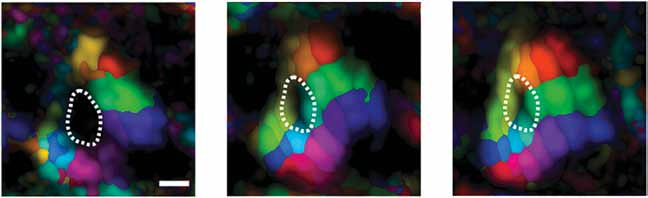
\includegraphics[keepaspectratio,width=0.7\textwidth]{99_images/keck-1-2a}
    \caption{Time lapse for a particular mouse - days 0, 11, 74}
  \end{figure}
  \begin{figure}
    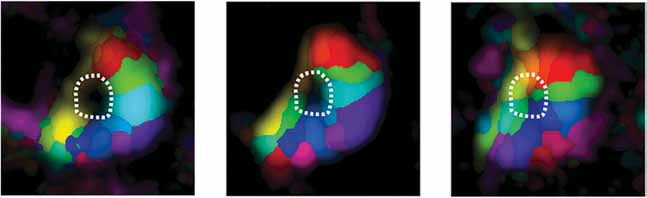
\includegraphics[keepaspectratio,width=0.7\textwidth]{99_images/keck-1-2c}
    \caption{Time lapse for a particular mouse - days 7, 12, 17}
  \end{figure}
\end{frame}
\begin{frame}{Results summary}
  \begin{itemize}
    \item Marked increases in turnover of of dendritic spines during functional reorganisation.
    \note[item]{Turnover - number of new and lost spines divided by twice the total number of spines}
    \item Almost complete replacement of set of spines on apical dendrites (91\% vs 38\% in control mice)
      \pause
    \item Turnover was as a result of an equal amount of spine loss and gain (evidenced by stable spine density) 
    \item Spine dynamics remained elevated for the first month, and returned to baseline levels after 2 months.
  \end{itemize}
\end{frame}
\begin{frame}{Results summary}
  \begin{itemize}
    \item Peri-LPZ, turnover was slightly elevated w.r.t. controls, but significantly lower than LPZ centre.
    \item Spine survival but not addition rates for peri-LPZ cells were lower than centre, thus, reorganisation progresses fastest in the centre.
      \pause
    \item No correlation between spine turnover and cortical depth.
    \item No change in dendritic architecture
  \end{itemize}
\end{frame}
\section{Paper 2 - inhibitory neurons}
\begin{frame}{Study}
  \begin{itemize}
    \item Dendrites on inhibitory neurons are typically smooth - dendritic spines conventionally believed to be absent
    \item A subset of inhibitory neurons have dendritic spines with excitatory synapses - which is what they study
      \pause
    \note[item]{It is well established that nearly all dendritic spines of excitatory neurons receive synaptic inputs}
    \item Confirmed that the majority of spines on the dendrites of inhibitory neurons carry synapses, and that most of these are from excitatory but not inhibitory, presynaptic neurons
    \item Also confirmed that dendritic spines of inhibitory neurons carry functional glutamatergic (excitatory) receptors.
    \note[item]{Using immunostaining}
  \end{itemize}
\end{frame}
\begin{frame}{Results - summary}
  \begin{itemize}
    \item Similar to excitatory neurons, in control animals, the inhibitory neurons show a stable spine density, and axonal bouton density over time.
      \pause
    \item Following lesions, a long lasting loss of excitatory spines on inhibitory neurons, and axonal boutons is observed in the LPZ.
    \begin{itemize}
        \item Initial rapid spine and bouton loss and no recovery of density 1 and 2 months after retinal lesion.
    \end{itemize}
  \end{itemize}
\end{frame}
\begin{frame}{Results - summary}
  \begin{itemize}
    \item Even inhibitory neurons whose cell body and dendrites were located outside the LPZ showed substantial decrease in spine and bouton density.
    \begin{itemize}
        \item For both, correlation between density and distance of cell body from border of LPZ
        \item Cells nearer to LPZ had similar densities, away from LPZ had densities similar to control animals
    \end{itemize}
  \end{itemize}
\end{frame}
\begin{frame}{Justification}
  \begin{itemize}
    \item changes reflect competition between lost and preserved visual inputs in the LPZ during functional reorganisation
      \pause
    \item simply reflect the overall reduction in cortical activity
      \pause
    \item can be distinguished by observing dynamics after \alert{complete} input removal
      \pause
    \item For excitatory neurons, structural dynamics of \alert{spines} increased after \alert{complete} input removal, but to a much lesser extent than during reorganisation following focal retinal lesions
    \begin{itemize}
      \item So, not simply due to reduction in activity, but also because of competition between deprived and non-deprived inputs.
    \end{itemize}
  \end{itemize}
\end{frame}
\begin{frame}{Justification}
  \begin{itemize}
    \item For both spines and boutons, density and survival fraction decreased to same degree after \alert{complete} input removal
    \begin{itemize}
      \item Suggesting that changes in density are largely driven by decrease in cortical activity
    \end{itemize}
  \end{itemize}
\end{frame}
\begin{frame}{Take away}
  \begin{itemize}
    \item Because the changes in inhibitory structures precede increases in excitatory spine turnover, these data suggest that inhibitory structural plasticity may be the first step in the cortical reorganisation after sensory deprivation
  \end{itemize}
\end{frame}
\section{My work - modelling}
\begin{frame}{Model}
  \begin{figure}
    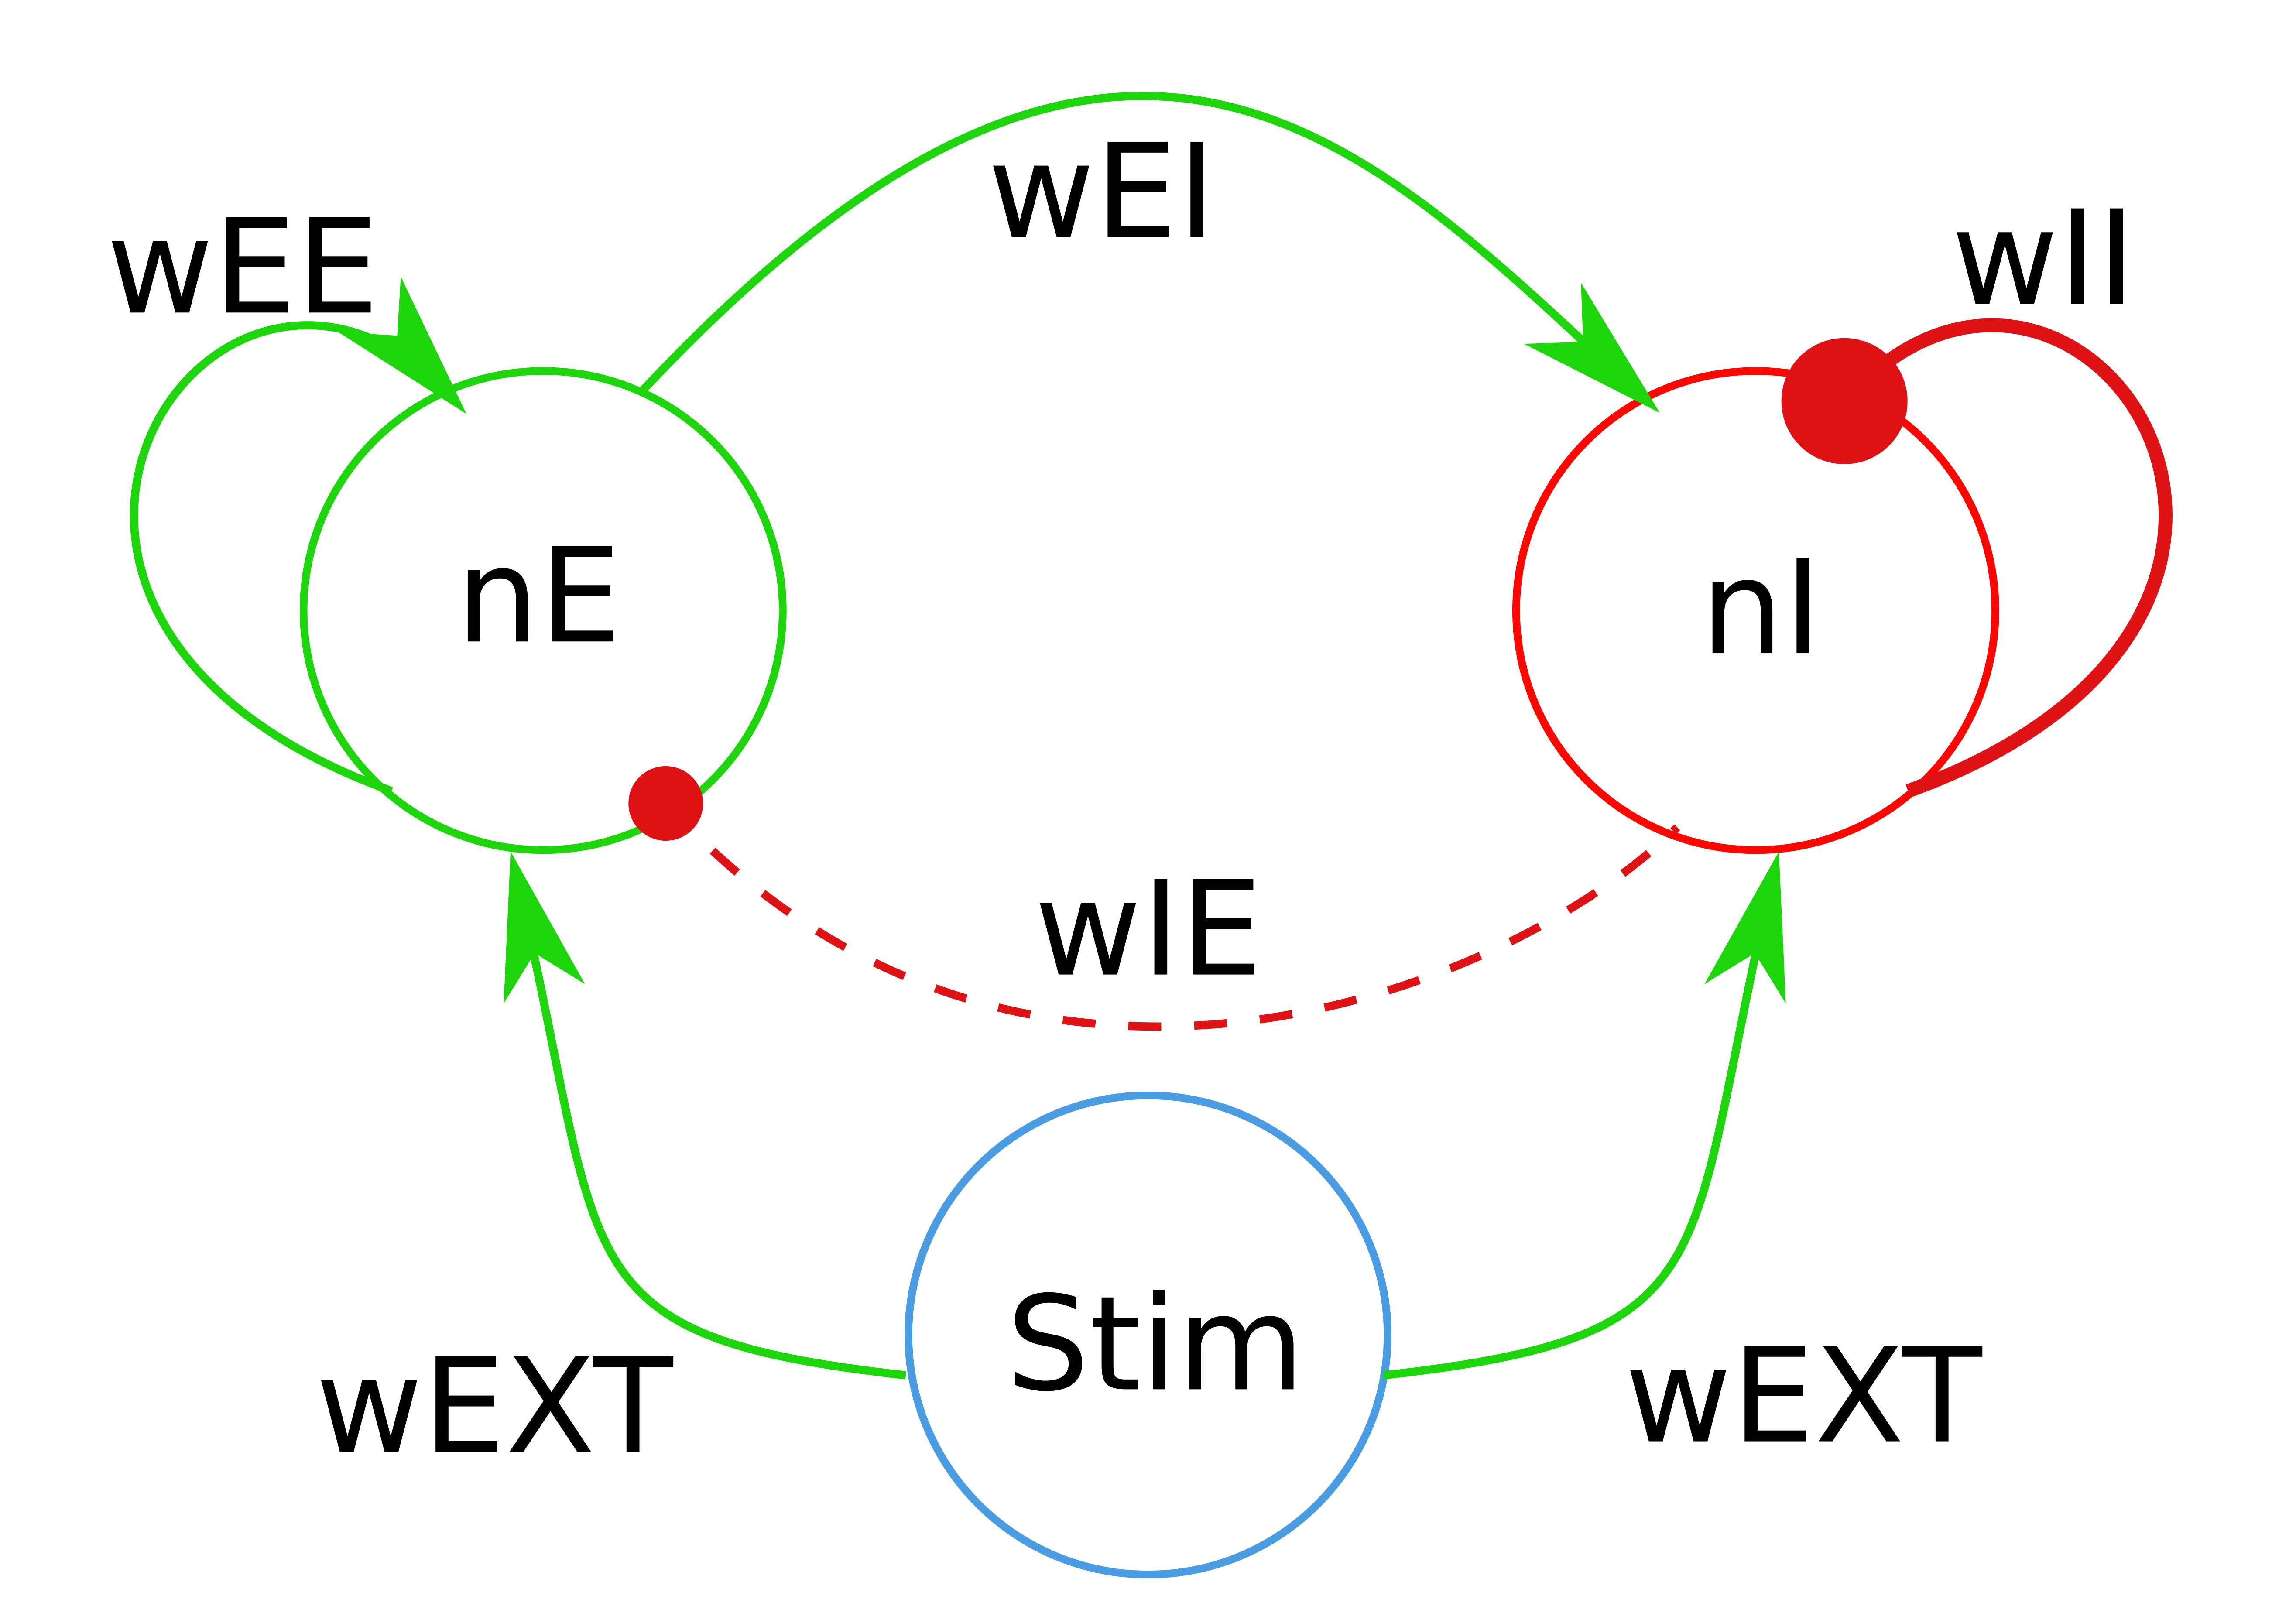
\includegraphics[keepaspectratio,width=0.7\textwidth]{99_images/model-schematic}
    \caption{Model schematic}
  \end{figure}
\end{frame}
\begin{frame}{Without repair - firing rates}
  \begin{figure}
    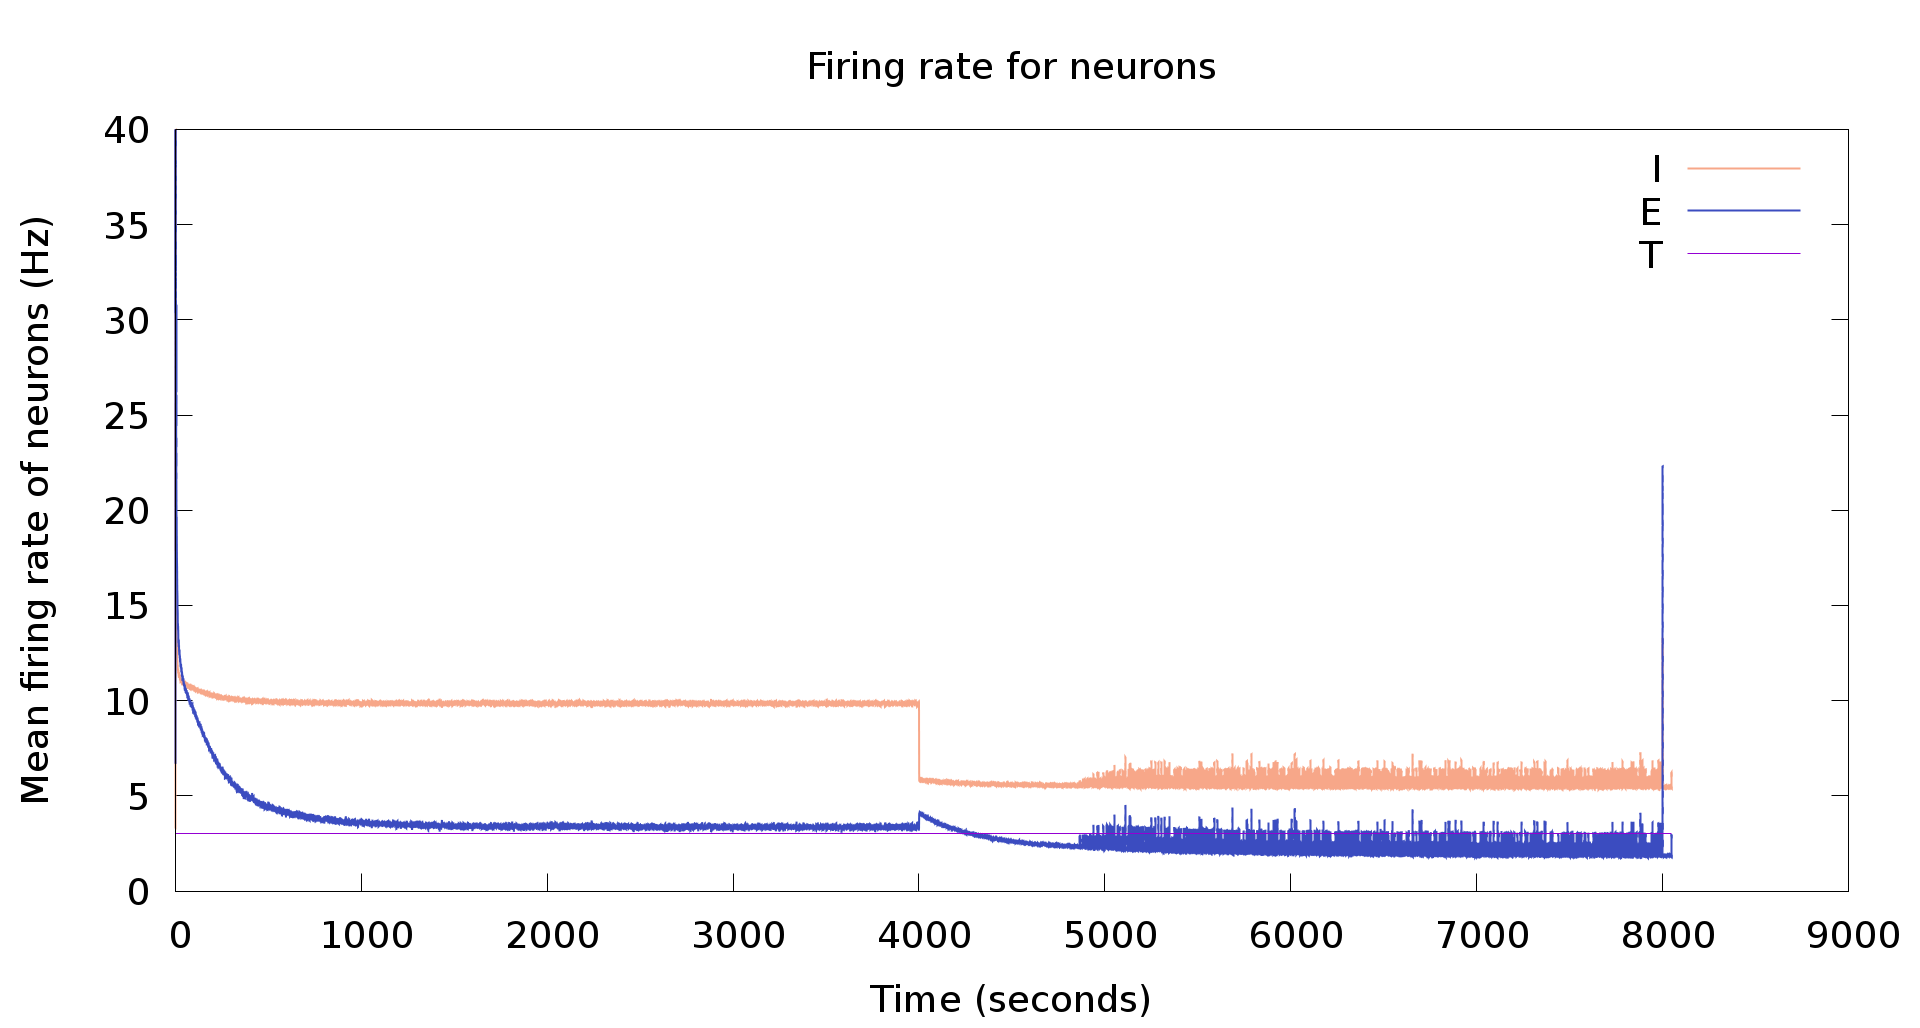
\includegraphics[keepaspectratio,width=0.8\textwidth]{99_images/201704272210-firing-rate-I-E-zoomed}
    \caption{Firing rates after lesion, without structural plasticity repair}
  \end{figure}
\end{frame}
\begin{frame}{Without repair - conductances}
  \begin{figure}
    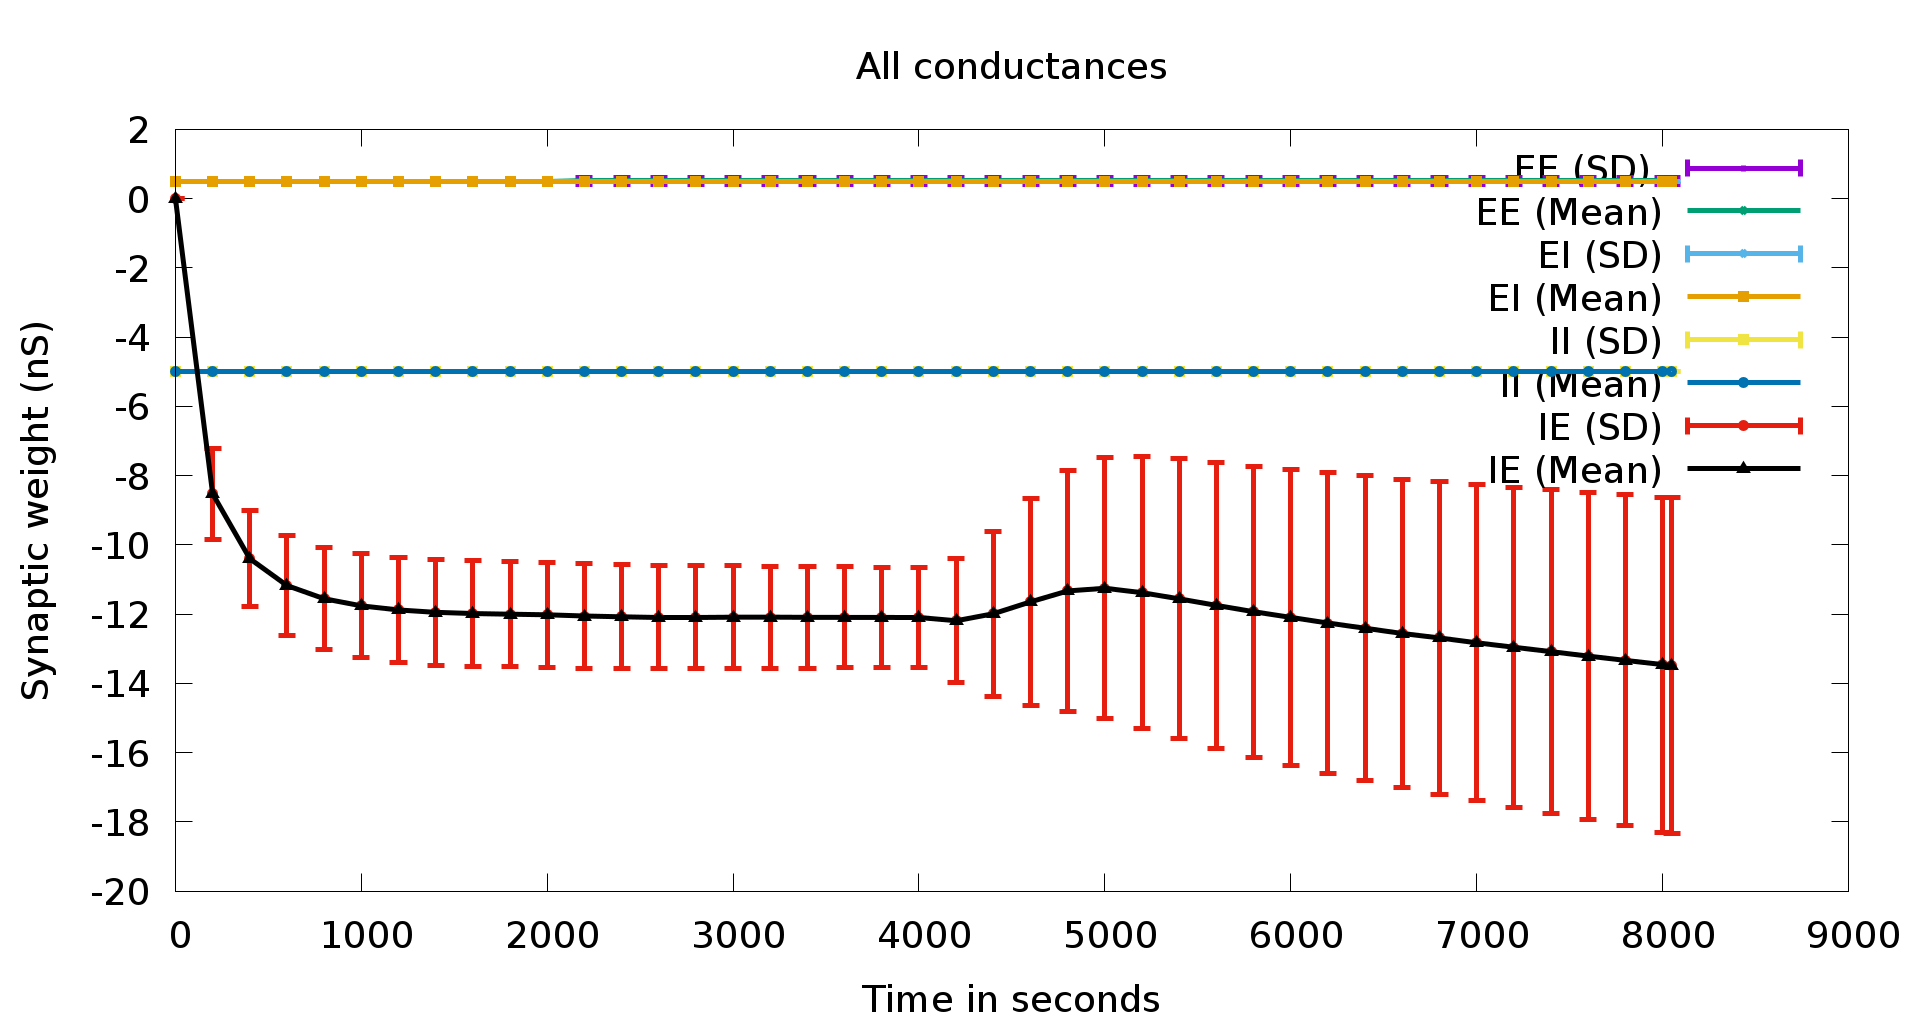
\includegraphics[keepaspectratio,width=0.8\textwidth]{99_images/201704272210-all-conductances}
    \caption{Conductances, without structural plasticity repair (negative conductance implies inhibitory)}
  \end{figure}
\end{frame}

\section*{References}
{\tiny
\begin{frame}[allowframebreaks]{References}
  \bibliographystyle{jneurosci}
  \bibliography{biblist}
\end{frame}
}
\begin{frame}
  \begin{center}
    \LARGE{Fin.}
  \end{center}
\end{frame}
\end{document}
